\chapter{Parking}
\label{ch:parking}
% ##################################################################################################################

\hfill \textbf{Author:} Rashid A. Waraich

\begin{center} 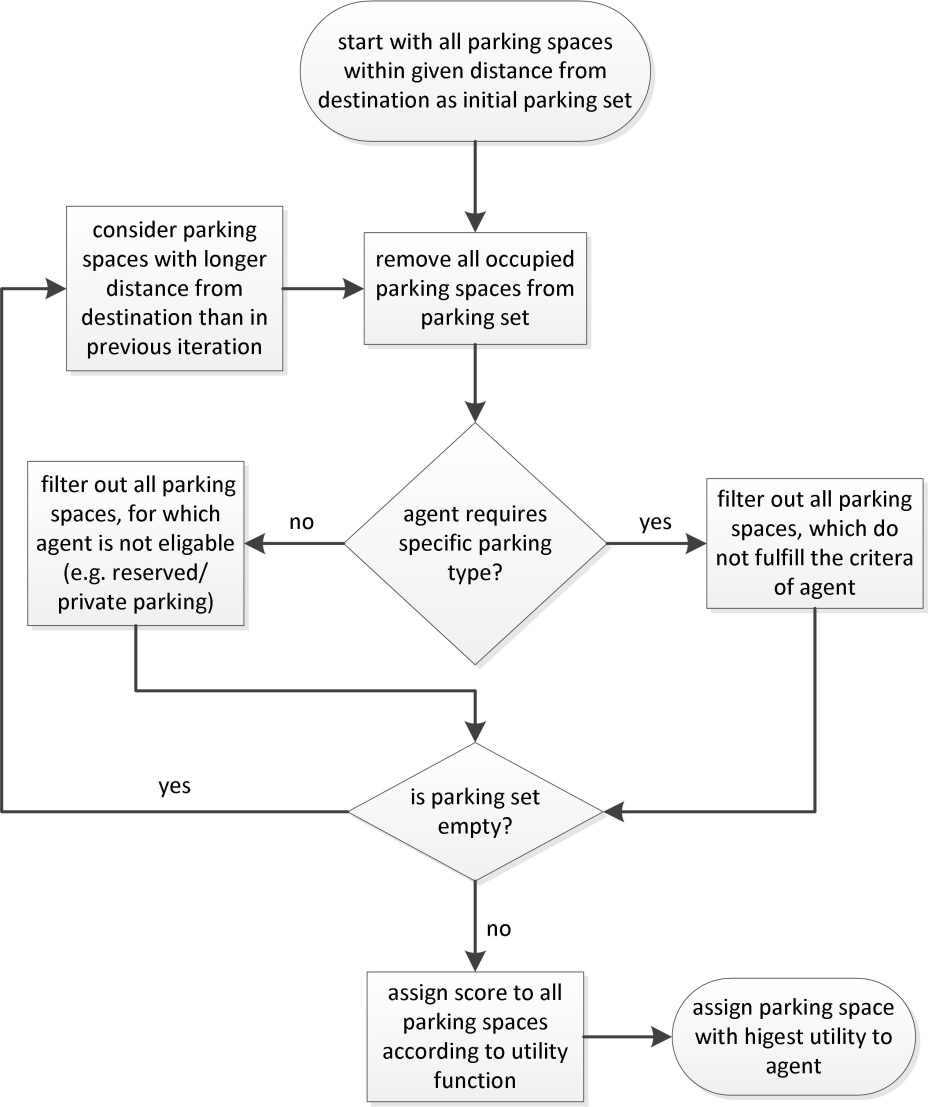
\includegraphics[width=0.4\textwidth, angle=0]{extending/figures/Parking/parking_algo.png} \end{center}

\editdone{This text has undergone the professional edit. Please no grammatical changes anymore! They are most-probably wrong.}

\createStandardInformation{parking}{org.matsim.contrib.parking.run.RunParkingExample}{parking}{\citet[][]{WaraichAxhausen_TRR_2012, WaraichEtAl_TechRep_IVT_2013_2, Waraich_unpub_Brownbag_2014, WaraichEtAl_unpub_STRC_2014}}

% \ah{see email by M. Balac, ``RunParkingExample'', 17.04.15}

%\kai{the RunParkingExample in contrib is not yet functional!!!!}

%\kai{References into playground should go.}

% ##################################################################################################################
\section{Introduction} 
The \gls{matsim} simulation, by default, does not consider parking infrastructure or supply constraints. However, this can lead to artificially high car traffic to city centers in the model, often not the case in the real world, due to limited parking. The modeling of parking is also important because traffic-related policies can be designed around parking; \eg raising  prices for parking at certain times of the day, or reducing parking supply in an area, can impact travel demand. 

This chapter describes work done to bridge this gap via parking models for \gls{matsim} .

% ##################################################################################################################
\section{Models}
For technical reasons, parking modeling efforts in \gls{matsim} were divided in two parts: parking choice and parking search, described in the following two subsections. 

% ==================================================================================
\subsection{Parking Choice Model}
The first approach for modeling did not change the \gls{matsim} traffic simulation; it extended it to capture parking supply through \lstinline|controler| \lstinline|listeners| and event handling. This means that no rerouting due to parking took place during the simulation. However, changed routes could be incorporated in a post-processing step, as described in \citet[][]{WaraichAxhausen_TRR_2012}. 

In the most general case, a parking choice model performed the following simulation steps; when a vehicle arrived at a destination in \gls{matsim}, the parking choice model assigned a parking spot in the agent's area, according to a customizable algorithm (\eg utility maximization). The assigned parking place was marked as occupied on arrival and became unoccupied again when the agent departed, allowing the model to simulate supply side constraints with the same temporal resolution as the basic \gls{matsim} model.

A simple parking choice model version was able to consider only walk distance minimization, ignoring other user preferences and park at the closest available public parking. A simple model like this was able to partially solve one of the main problems of the un-constrained parking model in \gls{matsim}; it made an area with little parking less attractive as a car destination due to longer walk distances. Parking model integration with \gls{matsim} was achieved by adding a term for the parking operation to the agent’s overall plan scoring function, as follows:

\begin{equation}
\label{eq:parkingutf}
S_{parking} = S_{walking} + S_{parking\ costs} + S_{parking\ search\ time}
\end{equation}

Beyond walking distance disutility, this scoring function could also include additional features like cost, or even estimated parking search times, using models like \citet[][]{HorniEtAl_IATBRspec_2013}.

A Zürich city study, which implemented a parking choice model and included trade-off between walk distance and parking cost, was presented in \citet[][]{WaraichAxhausen_TRR_2012}. This study also distinguished between public, private and reserved parking, where only certain people (\eg disabled) or certain vehicles could park (\eg electric vehicles). Figure~\ref{fig:parkingchoicealgo} shows parking choice models employed in this study, where a distinction between public, private and reserved parking was made. In \citet[][]{WaraichEtAl_unpub_TRB_2013}, another study for modeling parking in \gls{matsim} was reviewed, exploring individual gender and age parking preferences. Utility function parameters used in this study were based on a stated preference survey in Switzerland.

 % ------------
\createfigure%
{Parking choice algorithm}%
{Parking choice algorithm}%
{\label{fig:parkingchoicealgo}}%
{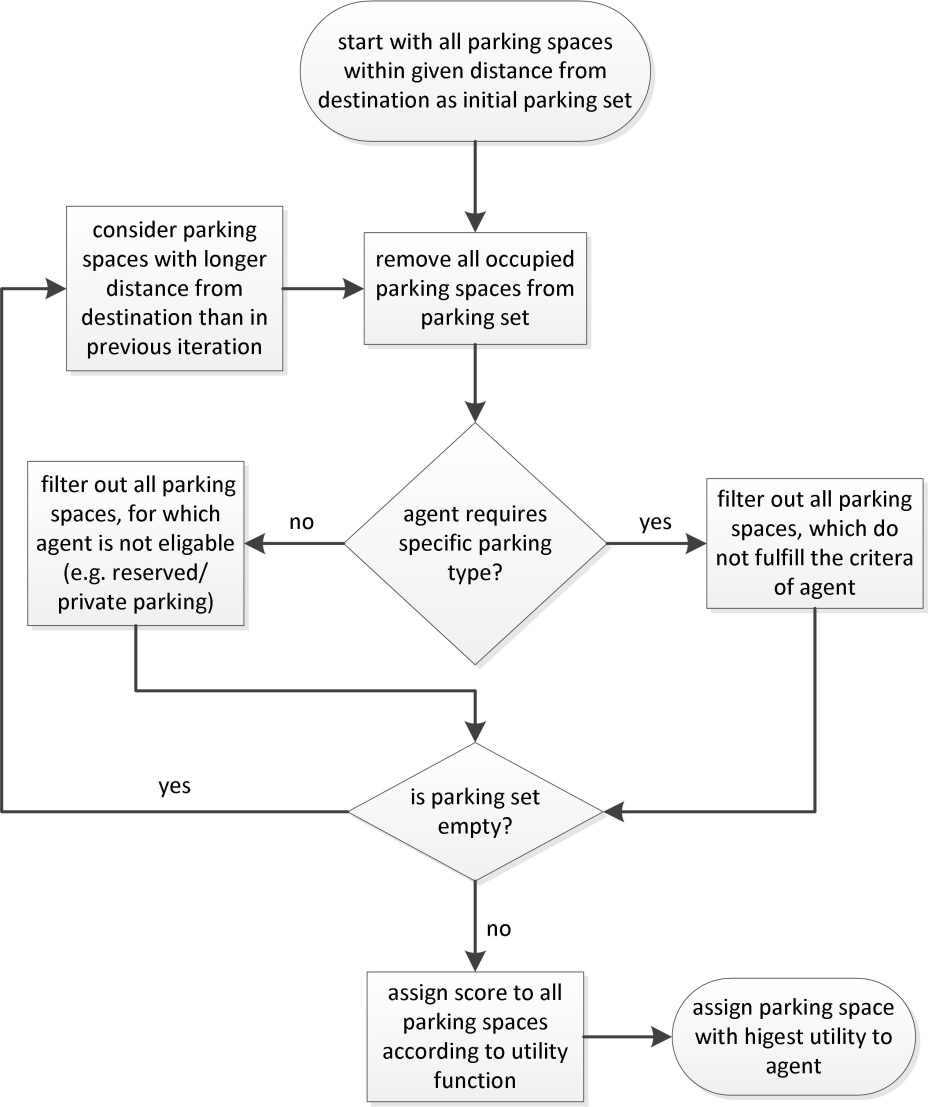
\includegraphics[width=0.8\textwidth, angle=0]{extending/figures/Parking/parking_algo.png}}%
{\citet[][]{WaraichAxhausen_TRR_2012}}
% ------------

% ==================================================================================
\subsection{Parking Search}
The parking choice model presented in the previous section could capture many relevant aspects of parking. However, it did not model parking search behavior;  studies conducted around the world suggest that, on average, around 30\,\% of city centers traffic could be due to parking search traffic \citet[][]{Shoup_RSUE_2004}. Thus, it seems extremely important to capture parking search related traffic in transportation models.

A first idea about model parking search traffic in \gls{matsim} was presented in \citet[][]{Waraich_unpub_IATBR_2012}. The basic idea came from surveys suggesting that people select certain strategies they think will be beneficial for them when starting the parking search process \citep[][]{AxhausenPolak_1989}. Proof of this concept for development was attempted, using within-day replanning (see Chapter~\ref{ch:withinday} and \citet[][]{DoblerEtAl_TRR_2012}). However, this path was aborted after development of several initial strategies, where performance and integration issues led to dead ends \citep[][]{WaraichEtAl_unpub_TRB_2013}; performance after optimization was around 24\,times slower than the original runs without parking operations. 

An alternative path closer to the idea presented in \citet[][]{Waraich_unpub_IATBR_2012} was successfully attempted, using a \gls{jdeqsim} based model (see Section~\ref{sec:using-jdeqsim}) with within-day support and travel time approximation, as seen in PSim (see Chapter~\ref{ch:psim}, \citet[][]{FourieEtAl_TRR_2013}). This removed overhead, present in the previous approach, enabling flexibility to implement many of the parking strategies presented in \citet[][]{AxhausenPolak_1989} and beyond. Publication of this approach's first results are expected in 2015.

Unfortunately, the approach is not available in packaged form to other users of \gls{matsim}. \kai{chk}

% ##################################################################################################################
\section{Applications}
Clearly, the parking model applications presented were important, diverse  and especially well-suited for policy design; one example of traffic policy design by means of targeted reduction of parking supply was presented in \citet[][]{WaraichAxhausen_TRR_2012}. \citet[][]{WaraichEtAl_unpub_TRB_2013} explained an application of performance-based pricing for parking in \gls{matsim}, where iteratively parking prices were adapted to match demand. An integration of parking choice and electric vehicle charging was presented in \citet[][]{WaraichEtAl_JanssensEtAl_2014} for a Zürich case study and \citet[][]{BemetzHohenfellner_BSCThesis_2014} described an even more sophisticated test model for parking and \gls{ev} charging, with various types of charging speed and prices.

% ##################################################################################################################
\section{Usage}
A general parking choice model was included in the parking \gls{contribution} of \gls{matsim}, which provided various extension interfaces; examples were included in the parking contribution to provide help with extension. 

% ##################################################################################################################


